\section{Diseño}
El módulo como proyecto de desarrollo enfocado a la metodología Ágil se encuentra dividido en varias épicas para partir en las funcionalidades.

Una épica se encuentra dividida en varias historias de usuario, donde las historias de usuario tienen el propósito de entregar valores de negocio al cliente en un periodo establecido de 2 semanas como sprint. Estas historias de usuario pueden ser a la vez divididas buscando la simplicidad de las historias donde cada una debe seguir la práctica INVEST de la metodología Ágil.

Cada historia puede estar compuesta de tareas que tienen como propósito servir al desarrollador como recordatorio de algunas labores pendientes a la hora de desarrollar la historia. Cada tarea debía tener un encargado, pero eso no significaba que esa persona debía hacer sola la implementación.

\begin{figure}[H]
\centering
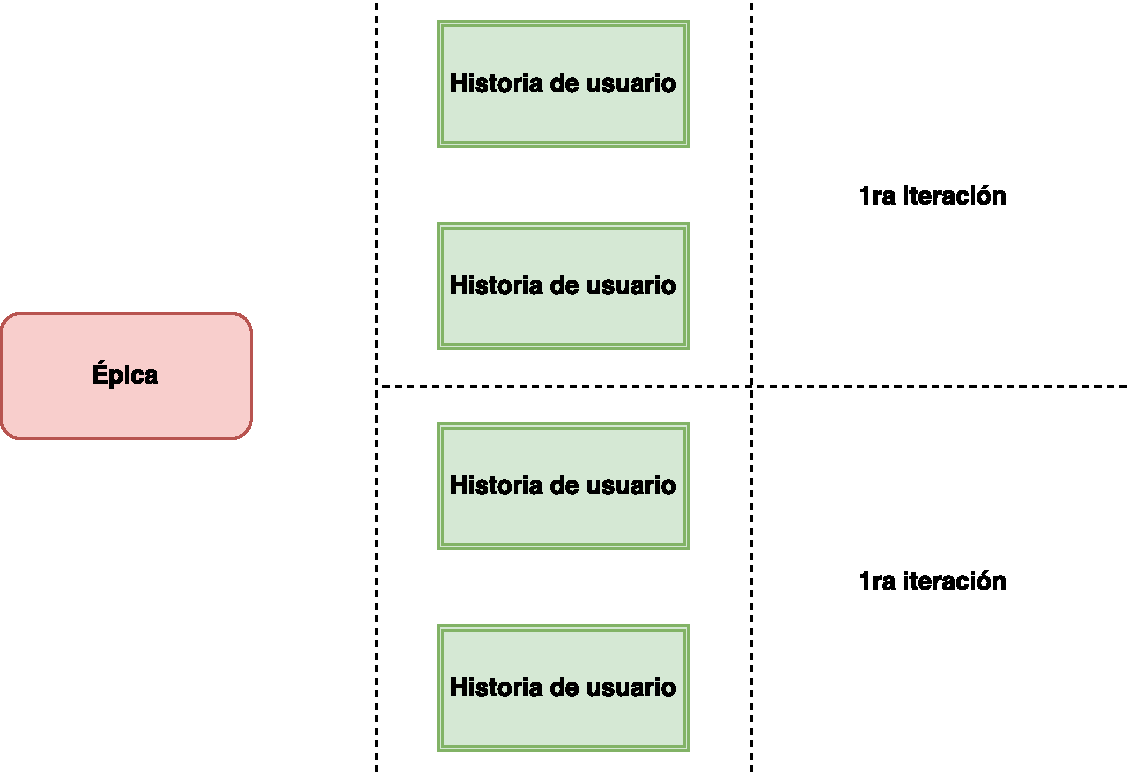
\includegraphics[width=125mm,scale=1]{Capitulos/PropuestadeSolucion/Imagenes/epic_diagram}
\caption{Diagrama de definición de épicas en la metodología ágil}
  \label{epic}
\end{figure}

El PO\footnote{de sus siglas en inglés, Product Owner, que significa en español dueño del producto.} se encarga de la creación de épicas e historias de usuario, en caso de que la historia sea muy grande para terminar en un solo sprint o iteración se vuelve a partir en historias más pequeñas. 

En el caso de estudio, cada sprint consta de 2 semanas de trabajo, donde los desarrolladores como equipo se comprometen a entregar cierto valor de negocio que ellos estiman poder terminar en dicho periodo. Sin embargo, en caso de que el equipo considere que la totalidad de historias no podrán ser entregadas antes de que termine el periodo se pasa al siguiente sprint o se achica la historia minimizando los criterios de aceptación y los restantes se agregan en otra historia de usuario para las siguientes iteraciones.

Cada equipo tiene un líder, donde cada líder tiene como rol ser la brecha que une al PO con los desarrolladores. El PO se reúne con el líder de cada equipo para verificar las prioridades de las historias de usuario que están pendientes en el backlog\footnote{Bolsa de historias de usuarios pendientes.}. 

En la figura \ref{workflow} se puede apreciar el ciclo de vida de las historias de usuario, donde una vez que es creada pasa al estado de \enquote{TODO}, que quiere decir que está pendiente a ser desarrollada. Una vez que un miembro del equipo de desarrollo comienza una historia o tarea pasa al estado de \enquote{IN PROGRESS} y cuando termina pasa al estado de \enquote{UNDER REVIEW}. 

En dicho estado se revisa la funcionalidad mediante validaciones de parte de los miembros del equipo de desarrollo y de parte del equipo de expertos en dominios de didáctica en universidades norteamericanas incluyendo a un PhD en educación, donde se deben cumplir los criterios de aceptación para que pase al estado de \enquote{CLOSED} que quiere decir que se terminó y que la historia fué aprobada.  

En caso de que la historia no consiga cumplir los criterios de aceptación correspondientes durante la validación se considera que la historia no está terminada y que debe pasar al estado de \enquote{REOPEN}, en este estado se puede pasar ya sea desde el estado \enquote{UNDER REVIEW} o si ya está en el estado \enquote{CLOSED}.

Cualquier otro problema o error de código que tenga la nueva funcionalidad se debe crear un ticket de error o bug especificando como reproducir el problema y el comportamiento esperado. En caso de no poder reproducir este comportamiento se pide más información al respecto o pasa al estado de \enquote{CLOSED} en caso de que el comportamiento ya no se pueda reproducir.

\begin{figure}[]
\centering
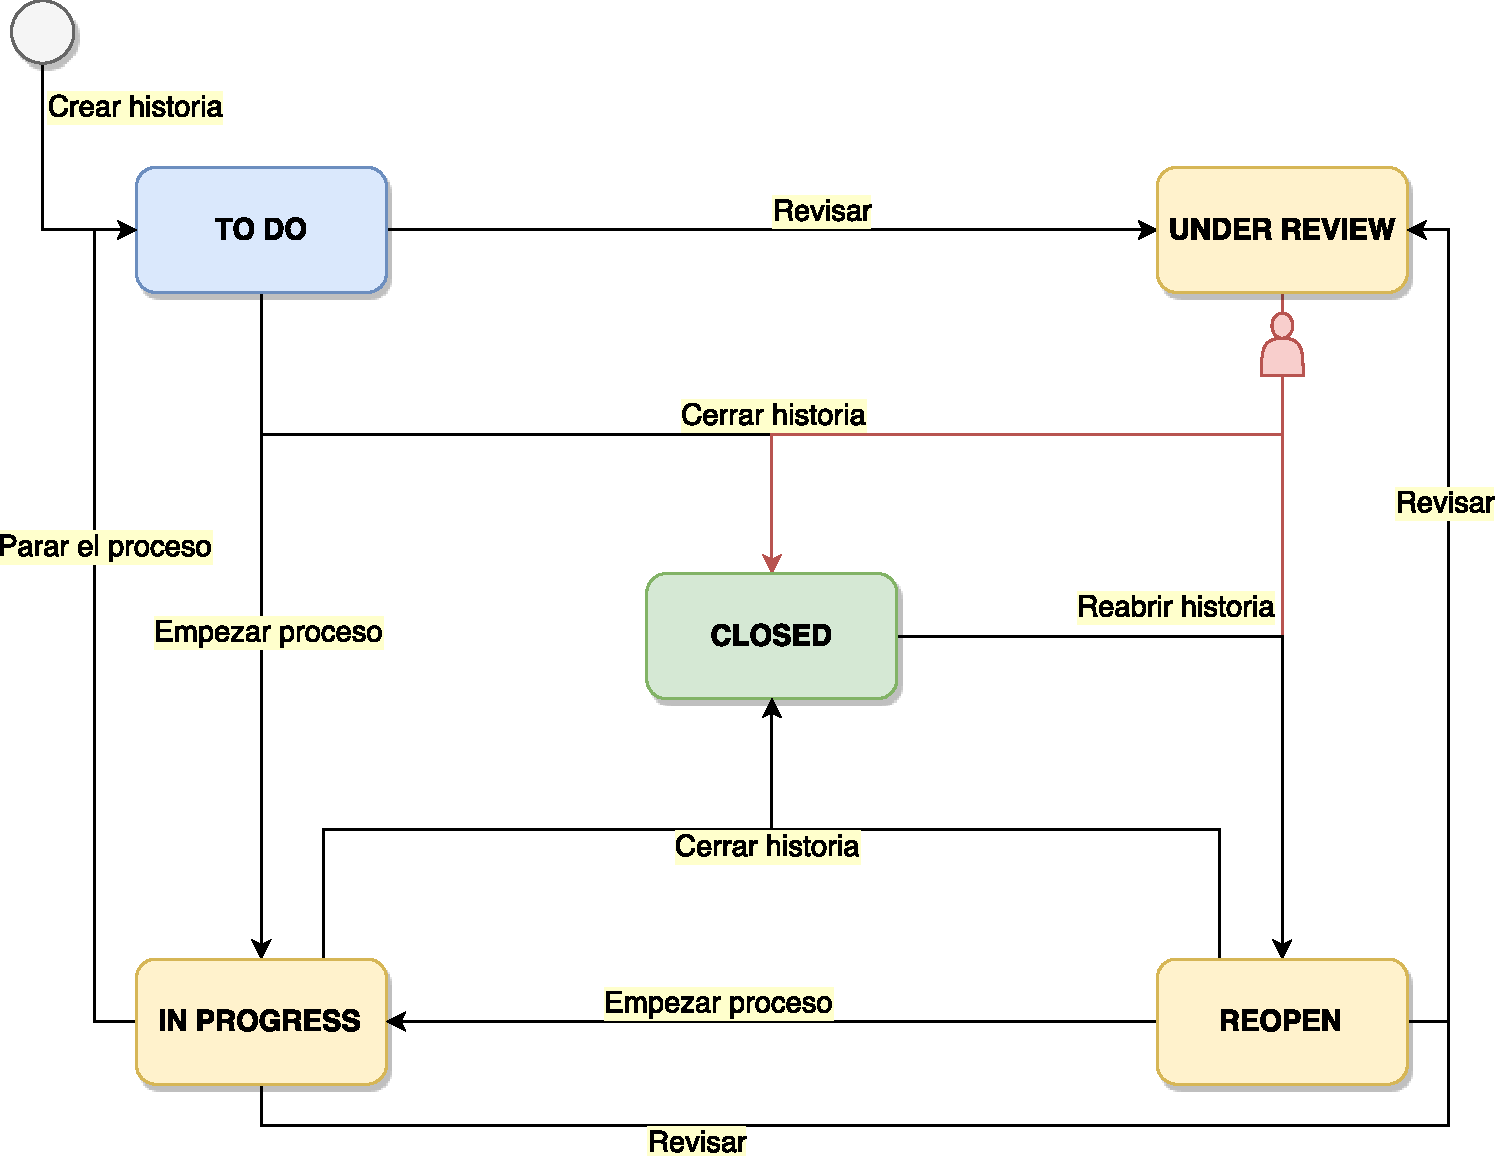
\includegraphics[width=125mm,scale=1]{Figuras/workflow}
\caption{Flujo de desarrollo de historias de usuario.}
  \label{workflow}
\end{figure}

Al inicio del diseño de la aplicación se llevará a cabo una serie de diseños de funcionalidad y usabilidad que llevar a la mejor experiencia de uso del módulo de gestión curricular, donde dichos diseños serán validados por el equipo en los Estados Unidos antes de iniciar el desarrollo.

\subsection{SCRUM}
Scrum es un proceso en el que se aplican de manera regular un conjunto de prácticas para trabajar colaborativamente, en equipo, y obtener el mejor resultado posible de un proyecto. Estas prácticas se apoyan unas a otras y su selección tiene origen en un estudio de la manera de trabajar de equipos altamente productivos.

En Scrum se realizan entregas parciales y regulares del producto final, priorizadas por el beneficio que aportan al PO. Por ello, Scrum está especialmente indicado para proyectos en entornos complejos donde se necesita obtener resultados con el mínimo esfuerzo y los requisitos son cambiantes o poco definidos. Además, en dichos ambientes la innovación, la competitividad, la flexibilidad, y la productividad son fundamentales.

Scrum también se utiliza para resolver situaciones en que no se está entregando al cliente lo que necesita, cuando las entregas se alargan demasiado, los costes se disparan o la calidad no es aceptable, cuando se necesita capacidad de reacción ante la competencia, cuando la moral de los equipos es baja y la rotación alta, cuando es necesario identificar y solucionar ineficiencias sistemáticamente o cuando se quiere trabajar utilizando un proceso especializado en el desarrollo de producto. 

\subsection{Proceso}
En Scrum un proyecto se ejecuta en bloques temporales cortos y fijos que los conocemos como sprints o iteraciones. Estas iteraciones por lo general duran 2 semanas aunque en algunos equipos son de 3 y hasta 4 semanas, límite máximo de feedback y reflexión\citep{davis_agile_2015}. Cada iteración tiene que proporcionar un resultado completo, un incremento de producto final que sea susceptible de ser entregado con el mínimo esfuerzo al cliente cuando lo solicite.

El proceso parte de la lista de objetivos o requisitos priorizada del producto, que actúa como plan del proyecto. En esta lista el cliente prioriza los objetivos balanceando el valor que le aportan respecto a su coste y quedan repartidos en sprints y entregas.

\begin{figure}[H]
\centering
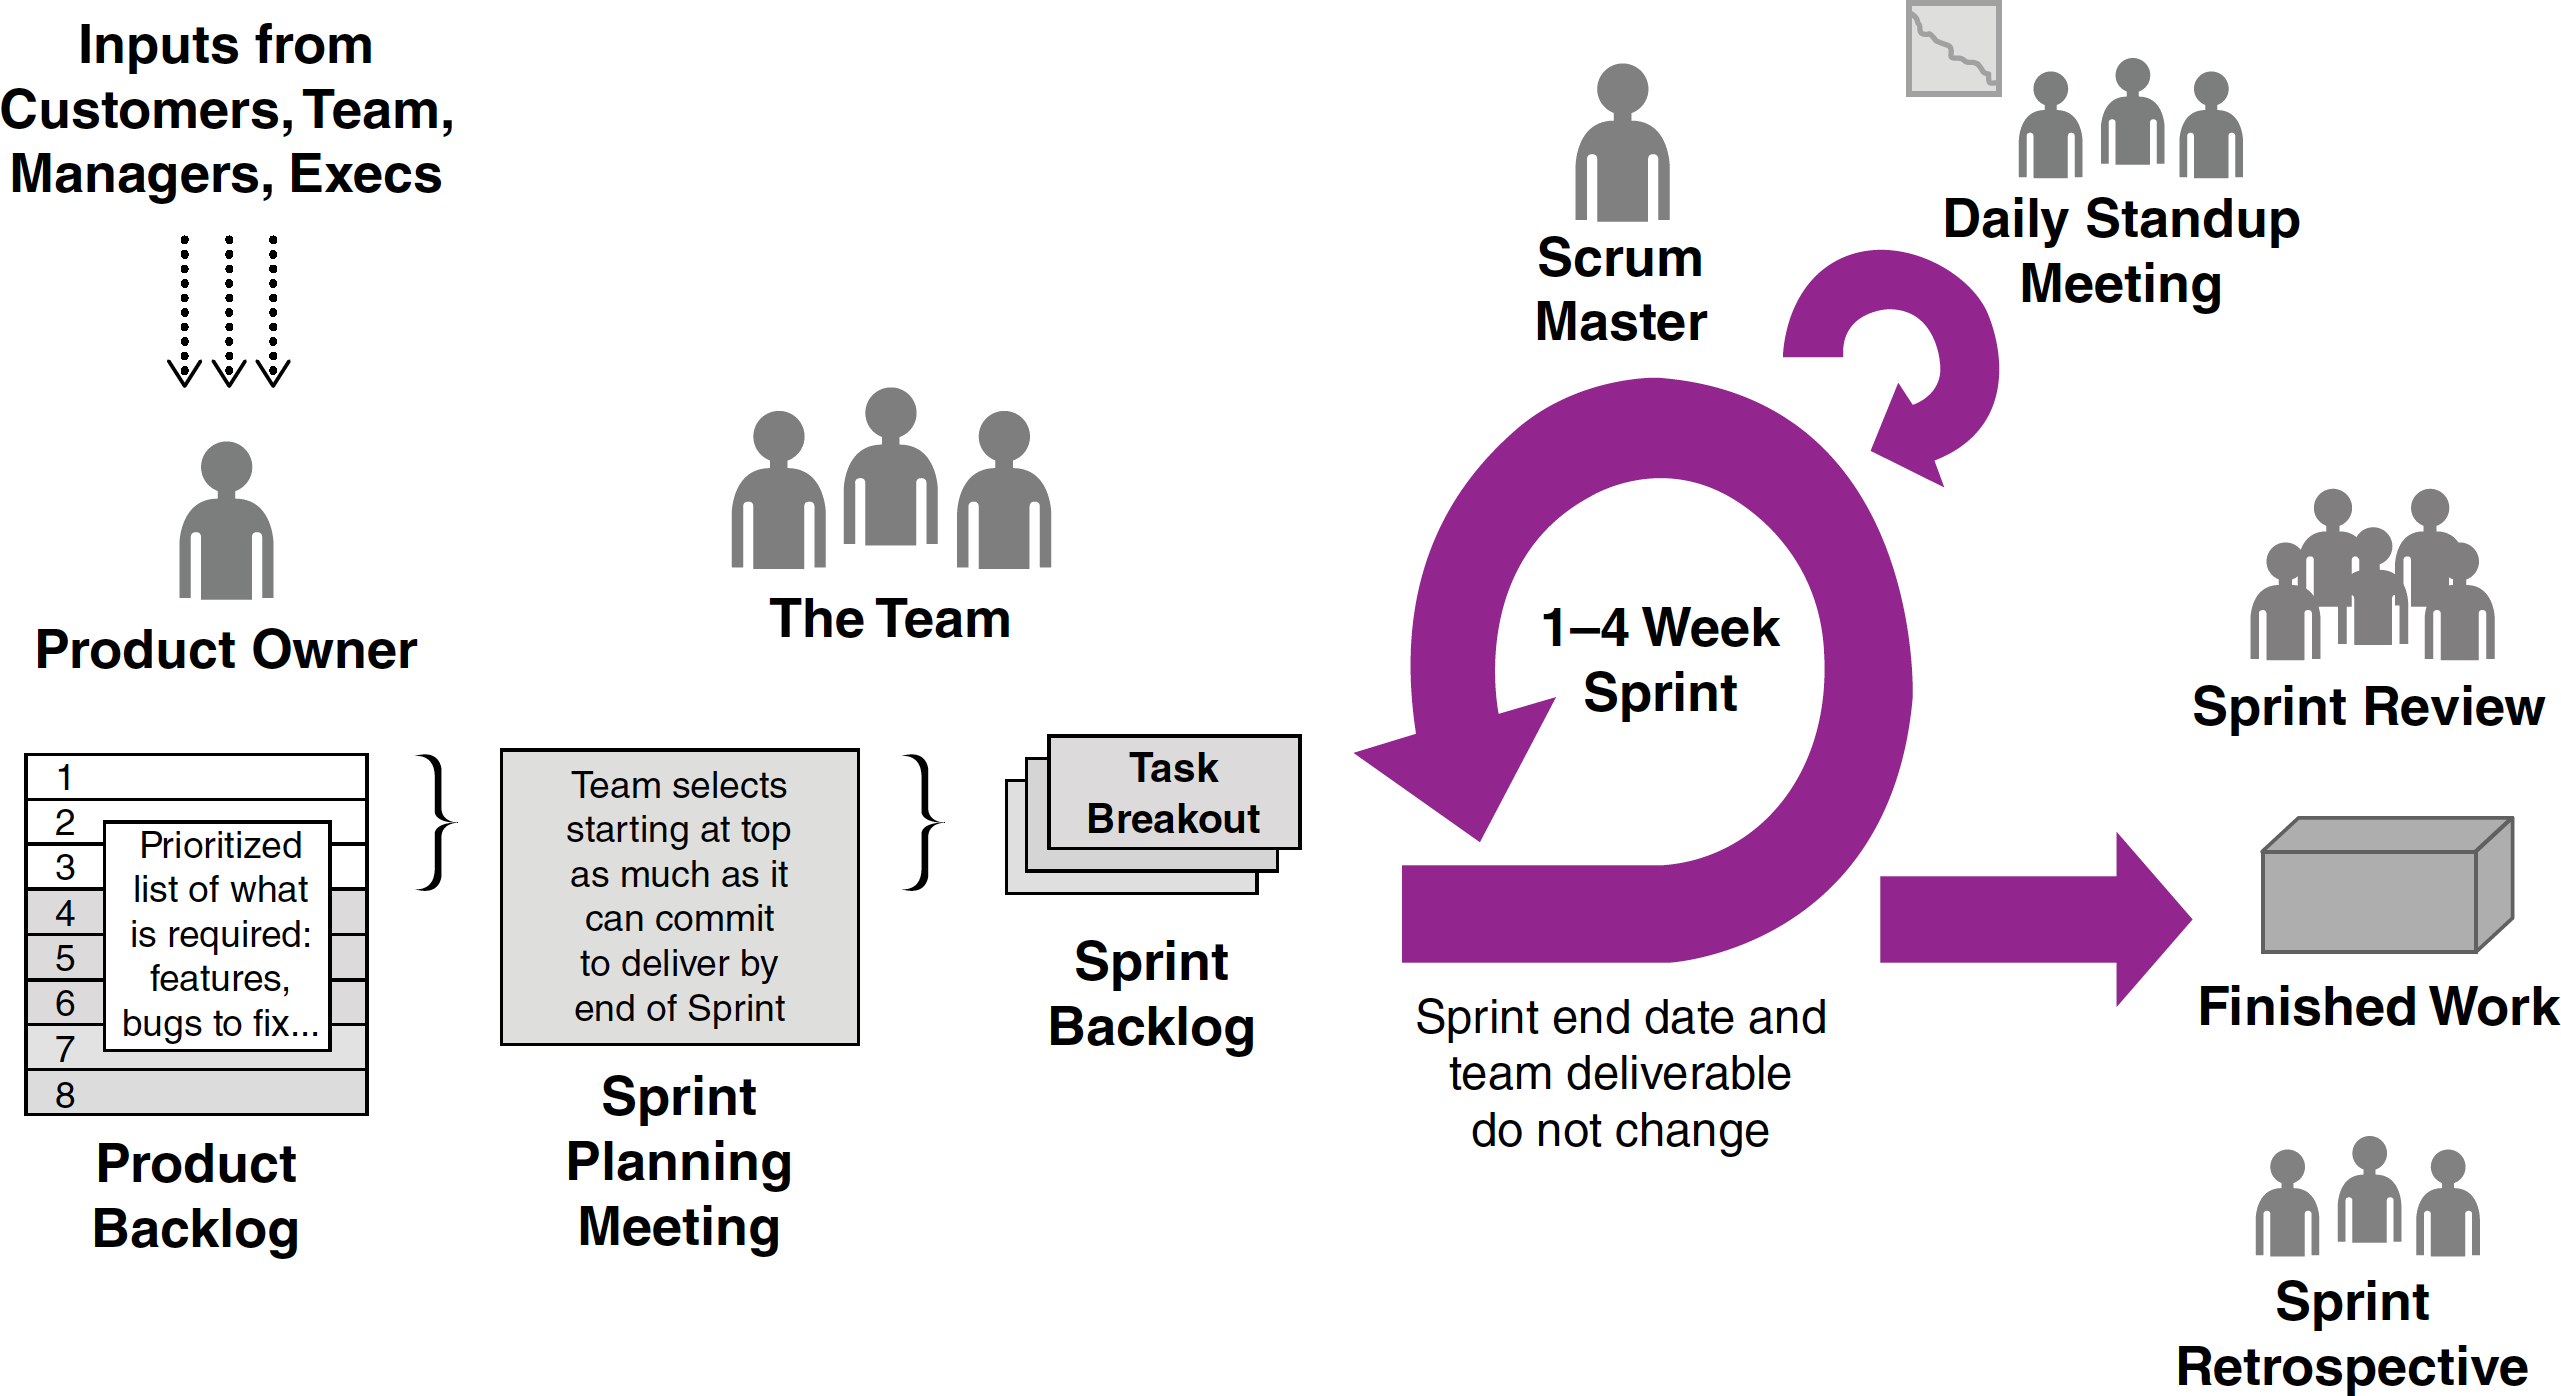
\includegraphics[width=125mm,scale=1]{Figuras/flujo_scrum}
\caption{Flujo de la técnica SCRUM.}
  \label{flujo_scrum}
\end{figure}

\subsection{Planificación de iteraciones}
El primer día de la iteración se realiza la reunión de planificación de la iteración y consta de dos partes:
\begin{itemize}
    \item \textbf{Selección de requisitos} (4 horas máximo) – El PO presenta al equipo la lista de requisitos priorizada del producto o proyecto. El equipo pregunta al PO las dudas que surgen y selecciona los requisitos prioritarios que se compromete a completar en la iteración, de manera que puedan ser entregados en caso de ser solicitados.
    \item \textbf{Planificación de la iteración o sprint} (4 horas máximo) – El equipo elabora la lista de tareas de la iteración necesarias para desarrollar los requisitos a que se ha comprometido. La estimación de esfuerzo se hace de manera conjunta y los miembros del equipo se asignan las tareas.
\end{itemize}

\subsection{Ejecución del Sprint}
El equipo realiza una reunión diaria (15 minutos aproximadamente). Cada miembro del equipo inspecciona el trabajo que el resto está realizando (dependencias entre tareas, progreso hacia el objetivo de la iteración, obstáculos que pueden impedir este objetivo) para poder hacer las adaptaciones necesarias que permitan cumplir con el compromiso adquirido. En la reunión cada miembro del equipo responde a tres preguntas:
\begin{itemize}
    \item ¿Qué he hecho desde la última reunión diaria?
    \item ¿Qué voy a hacer a partir de este momento?
    \item ¿Qué impedimentos tengo o voy a tener?
\end{itemize}
Durante la iteración el Scrum Master se encarga de que el equipo pueda cumplir con su compromiso y de que no se merme la productividad del equipo. Además, elimina los obstáculos que el equipo no puede resolver por sí mismo.

Durante el sprint, el PO junto con el equipo refinen la lista de requisitos para prepararlos para los siguientes sprints y, si es necesario, cambian o vuelven a planificar los objetivos del proyecto para maximizar la utilidad de lo que se desarrolla y el retorno de inversión.

\subsection{Inspección y adaptación}
El último día de la iteración se realiza la reunión de revisión del sprint la cual consta de dos partes:
\begin{itemize}
    \item \textbf{Demostración} (3 horas aproximadamente) – El equipo presenta al PO los requisitos completados en la iteración, en forma de incremento de producto preparado para ser entregado con el mínimo esfuerzo. En función de los resultados mostrados y de los cambios ocurridos en el contexto del proyecto, el PO realiza las adaptaciones necesarias de manera objetiva, ya desde la primera iteración, volviendo a planificar el proyecto.
    \item \textbf{Retrospectiva} (1 hora) - El equipo analiza cómo ha sido su manera de trabajar y cuáles son los problemas que podrían impedirle progresar adecuadamente, mejorando de manera continua su productividad. El Scrum Master se encargará de ir eliminando los obstáculos identificados.
\end{itemize}